% !Mode:: "TeX:UTF-8"
\section{问题描述}

某种药物在人体内的运转过程可用一个三房室系统描述，如题目所给示意图~\ref{fig:problem}。
\begin{figure}[H]
    \centering
    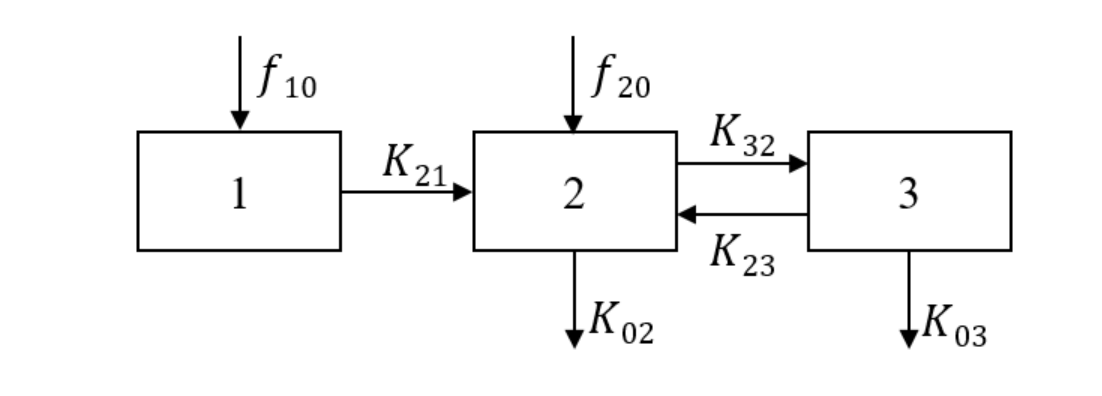
\includegraphics[width=0.8\textwidth]{figure/HW2figure/problem.png}
    \caption{三房室药物浓度随时间变化曲线}
    \label{fig:problem}
\end{figure} 
三个房室的体积均假定为 $1$ 个单位，因此房室内的药物质量即为药物浓度。设房室 $1$、$2$、$3$ 的药量（浓度）分别为 $x_1(t)$、$x_2(t)$、$x_3(t)$。药物输入与转运规则如下：
\begin{itemize}
    \item 单位时间内注入房室 $1$ 的药物质量为 $f_{10}$；
    \item 单位时间内注入房室 $2$ 的药物质量为 $f_{20}$；
    \item 药物从房室 $2$ 向房室 $1$ 的转运系数为 $k_{21}$，向房室 $3$ 的转运系数为 $k_{23}$；
    \item 药物从房室 $3$ 向房室 $2$ 的转运系数为 $k_{32}$；
    \item 药物从房室 $2$ 排出体外的转运系数为 $k_{02}$；
    \item 药物从房室 $3$ 排出体外的转运系数为 $k_{03}$。
\end{itemize}
给定参数：$f_{10}=1$，$f_{20}=10\,\delta(t)$，$k_{21}=0.5$，$k_{23}=0.1$，$k_{32}=0.4$，$k_{02}=0.2$，$k_{03}=0.3$。要求建立该房室系统的数学模型，并求解未来一段时间内三个房室的药物浓度变化曲线。
这里的$\delta (t)$为冲激(脉冲)函数。
\section{方法原理}

\subsection{模型假设}

为简化问题，本文做出以下假设：

\begin{itemize}
    \item 假设1~ 药物在房室间的传递是一阶的
    \item 假设2~ 药物的分布符合房室模型的其他特征
\end{itemize}

\subsection{数学模型建立}
根据房室间的\textbf{质量守恒关系}，可列写各房室药量变化的常微分方程组。设 $x_1$、$x_2$、$x_3$ 分别为房室 $1$、$2$、$3$ 的药物量，则
$$
\begin{cases}
    \frac{dx_1}{dt} &= f_{10} - k_{21}x_1 \\
    \frac{dx_2}{dt} &= f_{20}(t) + k_{23}x_3 +k_{21}x_1 - k_{32}x_2 - k_{02}x_2 \\
    \frac{dx_3}{dt} &= k_{32}x_2 - k_{23}x_3 - k_{03}x_3 \label{eq:dx3}
\end{cases}
$$
将给定参数代入，微分方程组变为：
$$
\begin{cases}
\frac{dx_1}{dt} &= 1 - 0.5x_1, \\
\frac{dx_2}{dt} &= 10\delta(t) + 0.5x_1 + 0.1x_3 - 0.6x_2, \\
\frac{dx_3}{dt} &= 0.4x_2 - 0.2x_3.
\end{cases}
$$
初始条件：
\begin{equation}
    x_1(0)=0,\quad x_2(0^+)=10,\quad x_3(0)=0.
\end{equation}

\subsection{数值求解方法}
上述常微分方程组可使用 MATLAB 的 \texttt{ode45} 求解器进行数值积分。\texttt{ode45} 基于显式 Runge--Kutta法，适用于非刚性问题。定义状态向量 $\bm{x}=[x_1;x_2;x_3]$，编写右端函数文件 \texttt{drug\_3comp.m}，并在主脚本中调用 \texttt{ode45} 计算时间区间 $[0,T]$ 上的解，最后绘制三条浓度曲线。

\section{MATLAB 运行结果及分析}

\subsection{仿真结果}
运行主脚本 \texttt{main.m}，得到三个房室在 $t\in[0,5]$ 内的药物浓度变化曲线，如图~\ref{fig:conc} 所示。

\begin{figure}[H]
    \centering
    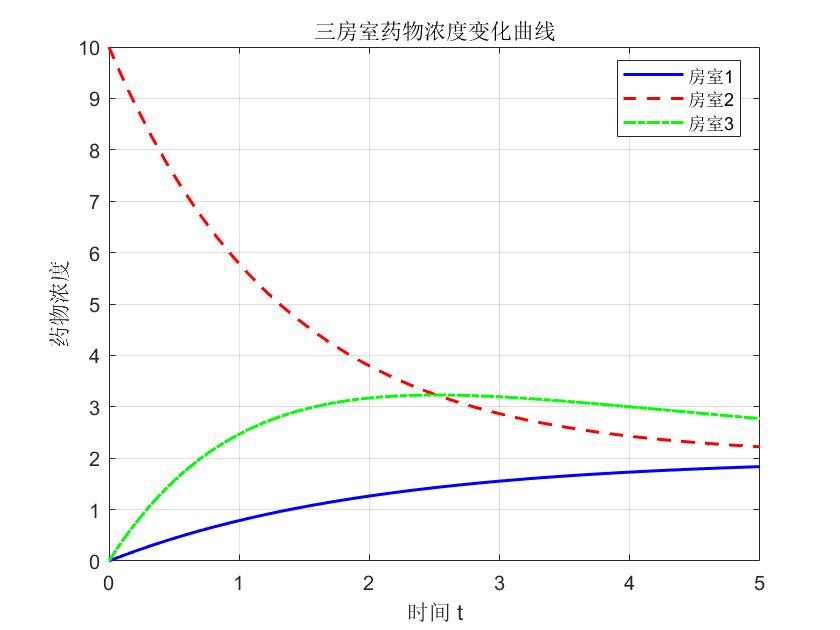
\includegraphics[width=0.8\textwidth]{figure/HW2figure/result.png}
    \caption{三房室药物浓度随时间变化曲线}
    \label{fig:conc}
\end{figure}
\par 
修改时间参数，还可以得到$t\in[0,10]$和$t\in[0,20]$的情况：
\begin{figure}[H]
    \centering
    \begin{minipage}[b]{0.4\textwidth}
        \centering
        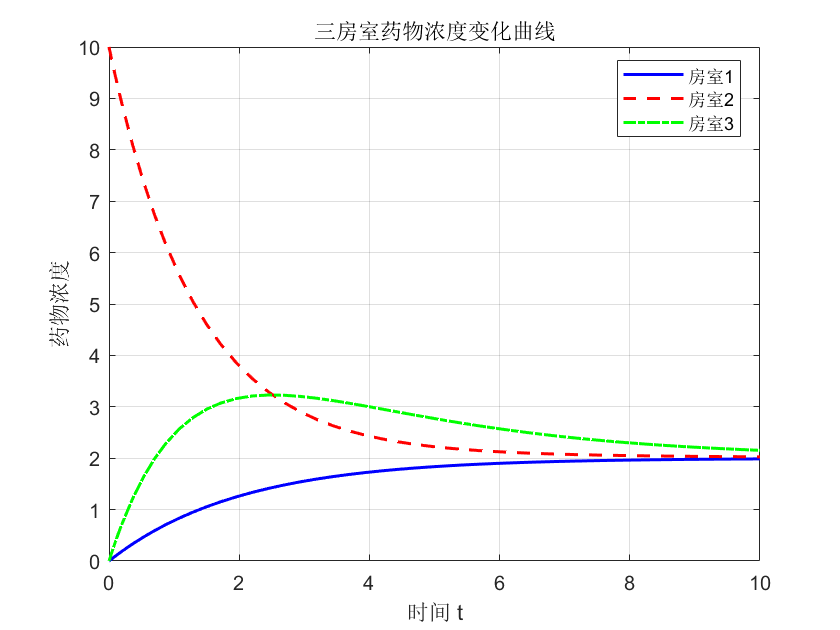
\includegraphics[width=\textwidth]{figure/HW2figure/t=10.png}
        \captionof{figure}{[0,10]下三房室药物浓度随时间变化曲线}
    \end{minipage}
    \hfill
    \begin{minipage}[b]{0.4\textwidth}
        \centering
        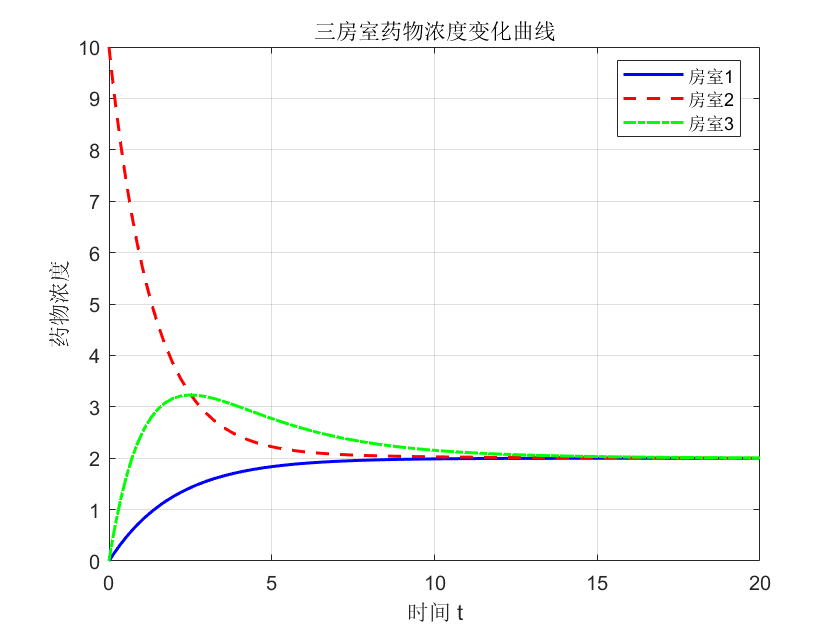
\includegraphics[width=\textwidth]{figure/HW2figure/t=20.png}
        \captionof{figure}{[0,20]下三房室药物浓度随时间变化曲线}
    \end{minipage}
\end{figure}

\subsection{结果分析}
从图~\ref{fig:conc} 中可观察到：
\begin{itemize}
    \item \textbf{房室 2}（红色虚线）：初始浓度为 $10$，由于药物向房室 $1$ 和房室 $3$ 转运以及自身排出，浓度迅速下降。约 $t=1$ 后下降速率减缓，并逐渐趋于零。这是因为没有持续的输入源（$f_{20}$ 为脉冲），且房室 $3$ 回流的量不足以维持较高浓度。
    \item \textbf{房室 1}（蓝色实线）：从零开始上升。初期因房室 $2$ 浓度高，$k_{21}x_2$ 项贡献较大，上升较快；随后上升速度减慢，但仍有恒速输入 $f_{10}=1$ 提供增长动力。最终$f_{10}$会和$x_2$主导的输出达成平衡。
    \item \textbf{房室 3}（绿色点划线）：从零开始先上升，在 $t\approx 2.5$ 时达到峰值，随后缓慢下降。这是因为初期 $x_2$ 浓度高，向房室 $3$ 的转运大于其自身消除速率；随着 $x_2$ 降低，消除占主导，浓度开始衰减。
\end{itemize}
整个系统的行为符合房室模型的动力学预期，并且参数设置使得房室 $2$ 的药量最终近乎清除，房室 $1$ 持续蓄积，房室 $3$ 出现先升后降的典型分布相特征。

\section{Simulink 运行结果及分析}
按照题目所给方程，建立simuink仿真模型如图~\ref{fig:simulink}所示：

\begin{figure}[H]
    \centering
    
\includegraphics[width=0.8\textwidth]{figure/HW2figure/simulink.png}
    \caption{本题建立的Simulink模型}
    \label{fig:simulink}
\end{figure} 
\par
这里，我们采用了Pulse~Generator，即阶跃（阶梯）函数来生成冲激（脉冲）函数。这是因为Simulink 无法直接产生理想的 Dirac $\delta(t)$ 函数，因此工程上常用窄而高、面积等于冲激强度的矩形脉冲来近似。只要脉冲宽度远小于系统主要时间常数（这里转运系数对应的时间尺度约 $1/0.8 \approx 1.25$ 时间单位），仿真结果就足够精确。我们在这里设置脉宽为 0.01、幅值 为1000 ，符合这一要求。

\subsection{仿真结果}
运行仿真脚本 \texttt{simulink.slx}，得到三个房室在 $t\in[0,5]$ 内的药物浓度变化曲线，如图~\ref{fig:SimulinkResult} 所示。

\begin{figure}[H]
    \centering
    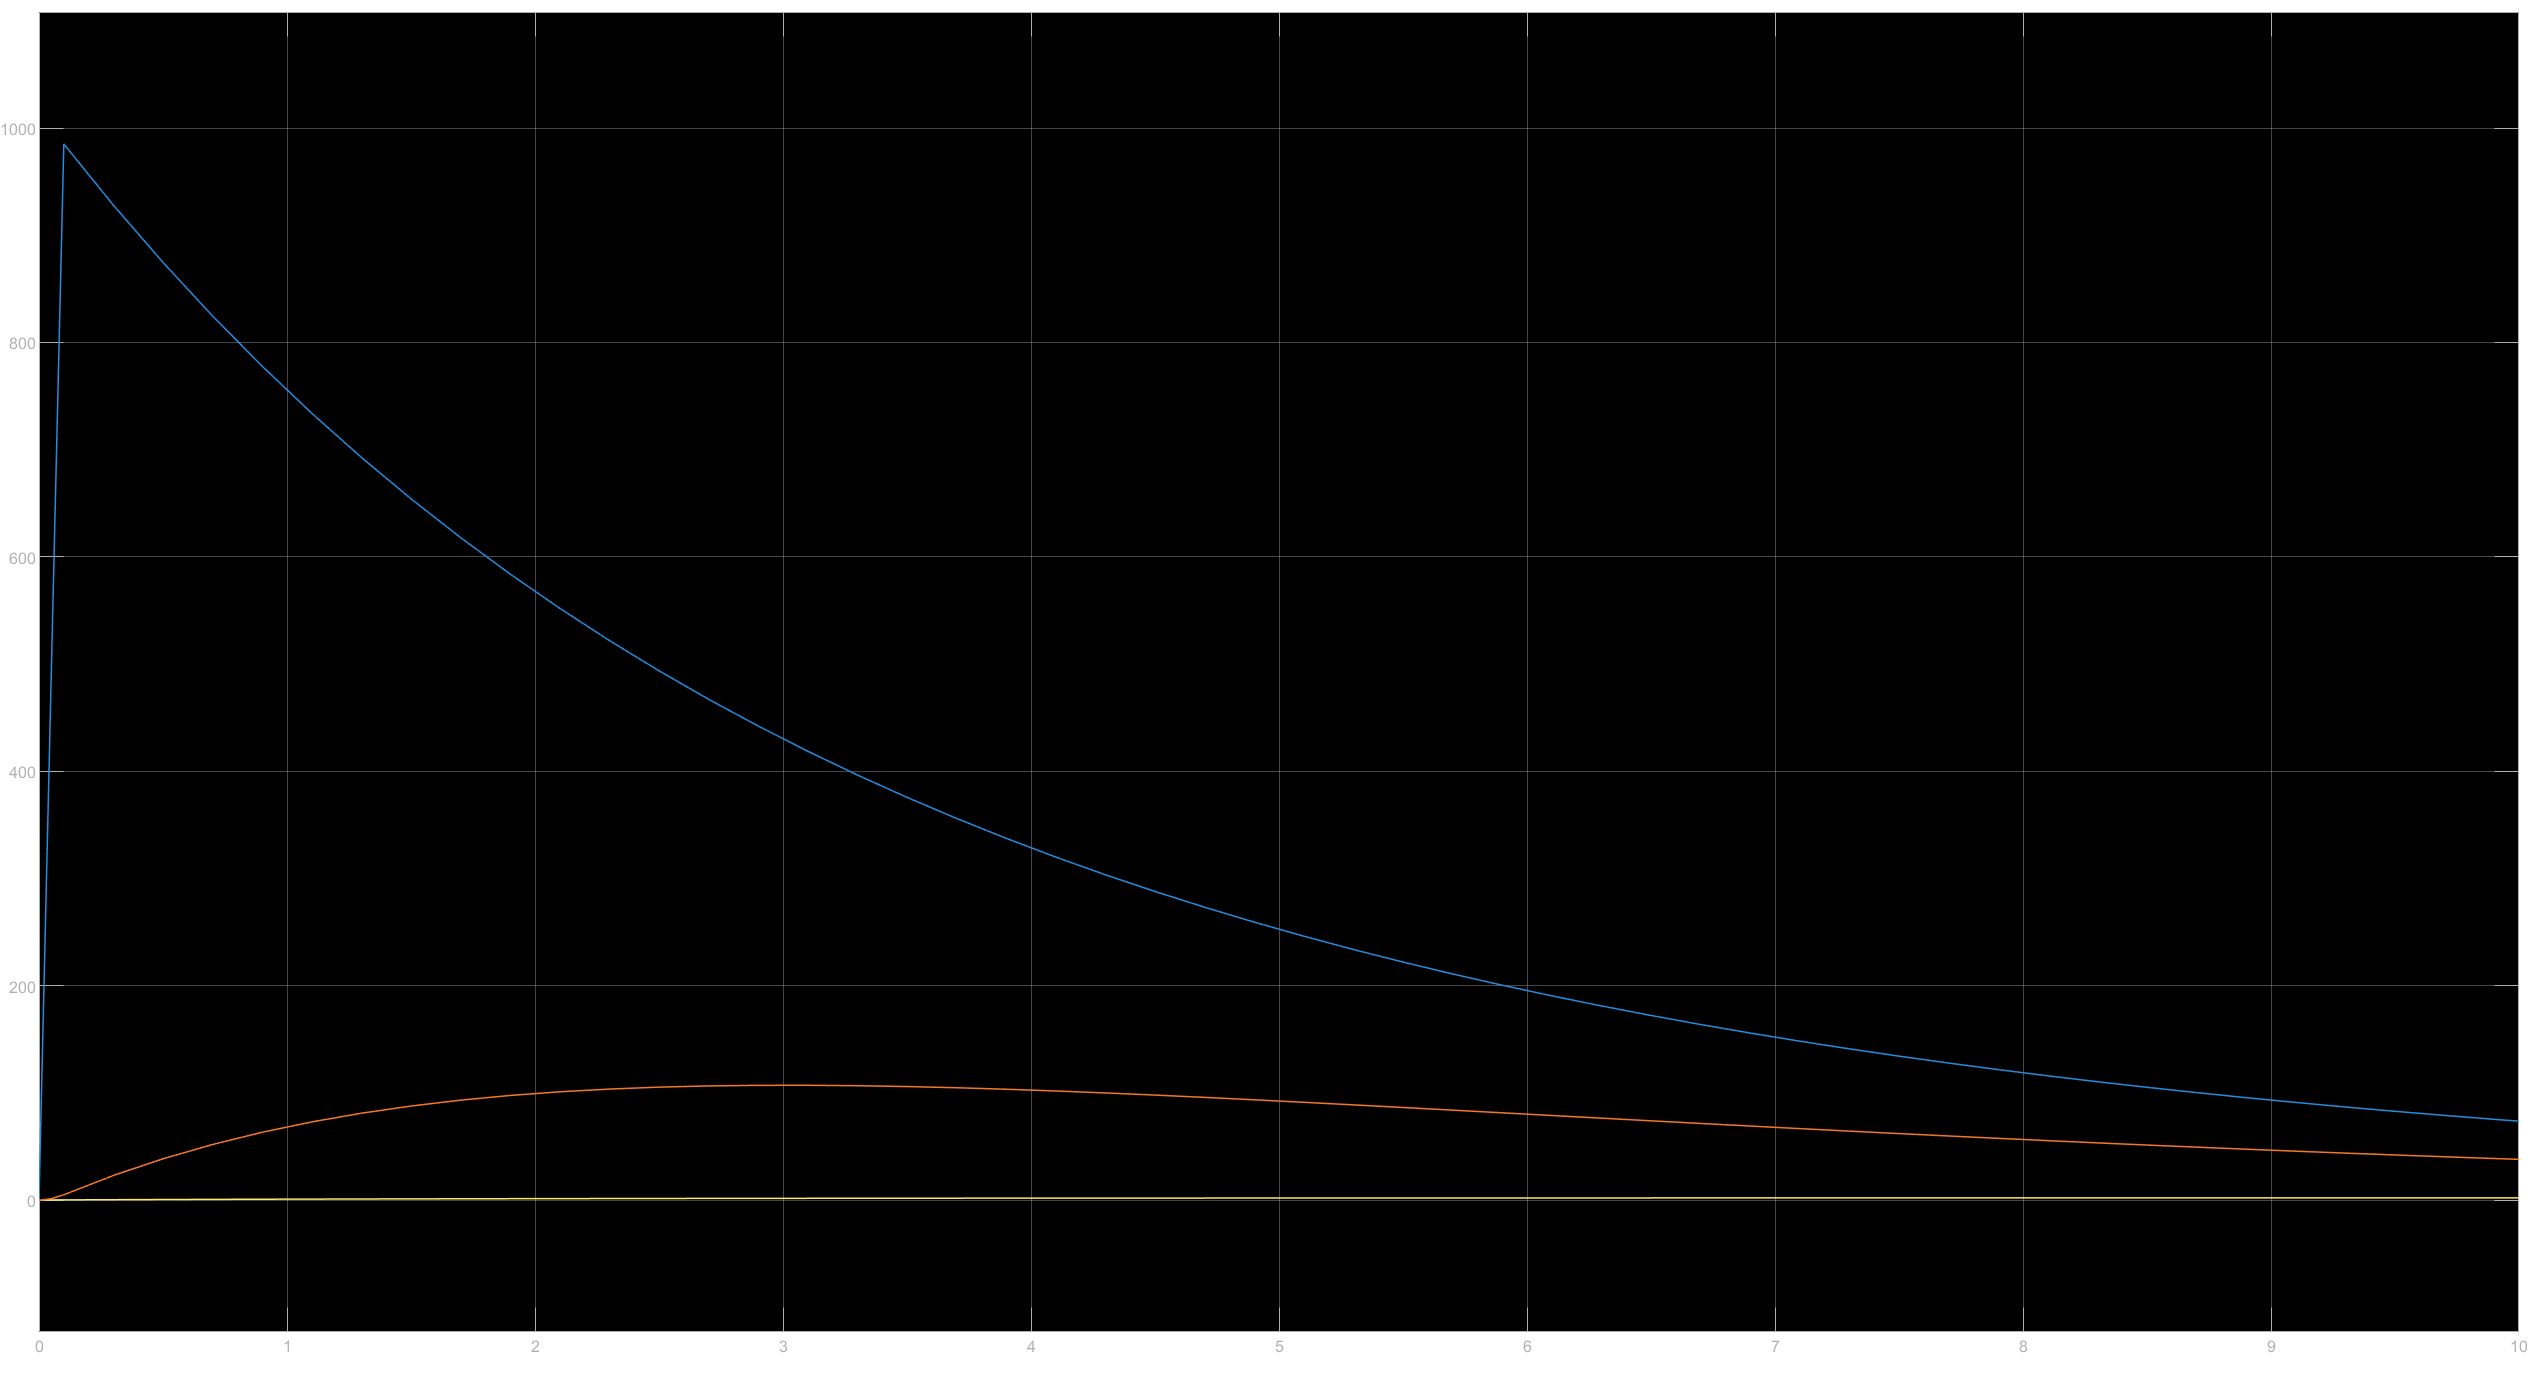
\includegraphics[width=0.8\textwidth]{figure/HW2figure/SimulinkResult.png}
    \caption{三房室药物浓度随时间变化曲线}
    \label{fig:SimulinkResult}
\end{figure} 

\section{结果讨论}

\subsection{模型合理性}
三房室模型能够较好地描述药物在体内吸收、分布、代谢的复杂过程。本三房室药物动力学模型构建符合药代动力学经典理论，严格遵循质量守恒定律，采用一阶线性动力学描述房室间药物转运及体外消除，与绝大多数小分子药物体内运转规律一致；房室划分贴合药物吸收、转运、代谢的生理路径，输入项与初始条件匹配给药特性，各转运、消除参数物理意义明确且符合实际，求解方法适配模型特性，能够准确刻画系统内药物浓度动态变化，模型具备充分的合理性与可靠性。

\subsection{参数影响}
改变各转运系数会显著影响曲线形态。例如：
\begin{itemize}
    \item 增大 $k_{21}$ 会加速药物从房室 $1$ 向房室 $2$ 的转移，使 $x_2$ 上升更快，同时 $x_1$ 衰减更快；
    \item 增大 $k_{02}$ 或 $k_{03}$ 会加快药物从系统消除，降低各房室浓度水平；
    \item 若 $f_{20}$ 不是脉冲而是持续输注，则房室 $2$ 将维持一定稳态浓度，系统行为完全不同。
\end{itemize}

\subsection{与 Simulink 仿真的对比}
题目要求使用 Simulink 求解，本文也同步额外采用了 MATLAB 脚本实现等效的数值求解。两种方法本质上都是对同一微分方程组的数值积分，结果应完全一致。Simulink 的优势在于图形化建模，便于直观理解房室间的流关系；而脚本方式更便于批量参数研究和结果后处理。

\subsection{结语}
在本文中，针对给定的三房室系统，建立了常微分方程模型，并用 MATLAB 进行了数值求解。仿真结果清晰地展示了各房室药物浓度的动态变化规律，验证了模型的正确性。该模型可为类似药代动力学问题的分析提供参考。

\section{代码附录}
\inputMATLAB{codes/HW2codes/main.m}
\inputMATLAB{codes/HW2codes/drug_3comp.m}